%qqqqqqqqqqqqqqqqqqqqqqqqqqqqqqqqqqqqqqqqqqqqqqqqqqqqqqqqqqqqqqqqqqqqqqqqq
%Quote
\begin{savequote}[50mm]
‘‘All the effects of Nature are only the mathematical consequences of a 
small number of immutable laws’’
\qauthor{Pierre Simon Laplace}
\end{savequote}
%qqqqqqqqqqqqqqqqqqqqqqqqqqqqqqqqqqqqqqqqqqqqqqqqqqqqqqqqqqqqqqqqqqqqqqqqq




%#########################################################################
\chapter{Computational Methods in Cosmology}
\label{cha:N-BodySimulations}


%Reviewed
In recent years, computational physics has acquired an important role in
physics, allowing modelling a lot of high-complexity systems without the
necessity of recurring to experiments and/or observations. Among the methods
covered by computational physics is highlighted the N-body problem since 
many phenomenons require the computation of the interactions between a
large number of bodies. Some illustrative examples of this are the 
modelling of molecular systems, plasma physics and specially gravitational
problems in astrophysics. The development of specific methods to solve 
this type of problems precedes the advent of computer systems, even so, 
their development has powered enormously this discipline such that it is
considered a new branch of physics.


%Reviewed
In this chapter will be covered in detail some specific methods for solving
gravitational problems in astrophysics, specially those related with 
simulations of the large-scale universe in the non-linear regime, ranging 
from basic algorithms to compute forces, methods to detect dark halos, to
basic classification schemes for the cosmological environment.

 

%#########################################################################




%*************************************************************************
%N-body Simulations
\section{N-body Simulations}
\label{sec:N-bodySimulations}


%Reviewed
Generally, the most suitable type of phenomena that can be modelled through 
N-body simulations is those where the interactions are strongly correlated 
between the constituent particles, such as long-range forces or non-local 
interactions. Figure \ref{fig:NbodyProblem} illustrates an arbitrary set 
of point particles which interact each other under the influence of a 
force field $\bds f$. Those conditions shape the classical formulation of 
the N-body problem.


\
%Reviewed
%.........................................................................
%N-Body Problem
\begin{figure}[htbp]
	\centering
	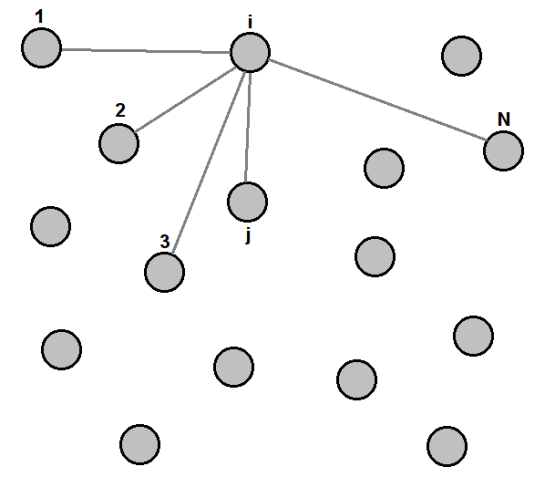
\includegraphics[width=0.50\textwidth]
	{./figures/3_nbody_simulations/Nbody_Problem.png}

	\caption{\small{Formulation of the N-body problem.}}
	
	\label{fig:NbodyProblem}
\end{figure}
%.........................................................................


%Reviewed
Assuming interactions that depends on the position\footnote{ In the 
generalized problem, interactions can depend on other parameters like 
the velocity or intrinsic degrees of freedom like the spin.}, it is 
obtained the below equation of movement of the $i$-th particle shown in 
the Figure \ref{fig:NbodyProblem} \cite{pfalzner1996} \cite{binney2008} 


%Reviewed
%.........................................................................
%Movement Equation
\eq{eq:MovementEquation}
{ \ddot{ \bds r}_i = \sum_{j=1}^N \bds f( \bds r_i, \bds r_j ) = -\nabla 
\phi( \bds r_i )\ \ \ \ \ \ \ i=1,2,\cdots,N }
%.........................................................................
where it has been introduced the potential function $\Phi(\bds r)$. For
the case of gravitational interactions, the potential acquires the form



%.........................................................................
%Gravitational Potential
\eq{eq:GravitationalPotential}
{ \phi(\bds r) = -\sum_{j=1}^N  \frac{G m_j}{|\bds r - \bds r_j|} }
%.........................................................................


%Reviewed
The general solution to the problem is obtained from the set $\{ \bds 
r_1(t),\cdots, \bds r_N(t) \}$, which is determined from the equations
\ref{eq:MovementEquation}. For this it is necessary to implement numerical
approximations due to the non-solvable (analytically) nature of the 
problem.



	%---------------------------------------------------------------------
	%Direct sum
	\subsection{P-P Method}
	\label{subsec:PPMethod}
	%---------------------------------------------------------------------
	
	
%Reviewed
The first approximation to find a solution of the equations of movement
\ref{eq:MovementEquation} is to compute all the $N-1$ interactions of the
$i$-th particle with all of the others in a specific time $t$ and this for
$i=1,2,\cdots N$, then, from a numerical integration scheme it is 
calculated the positions in a discretized later time $t+\Delta t$ and thus
until a given maximum time $t_{\submath{max}}$. This method is called P-P 
(Particle to Particle) and is one of the three standard methods for 
solving the N-body problem.


%Reviewed
When interactions present singularities, such as Coulombic potentials in
electrostatic and gravitational problems (equation 
\ref{eq:GravitationalPotential}), the integration of the equation of 
movement is very sensitive to close encounters between particles and 
therefore the resolution of the time step must be increased, thereby 
implying a considerable increasing of the computing time. A standard 
solution is to introduce a softening parameter that removes these 
singularities, but at the cost of losing accuracy in the solution. For the
gravitational potential \ref{eq:GravitationalPotential}, this leads to


%Reviewed
%.........................................................................
%Gravitational Potential
\eq{eq:SoftPotential}
{ \phi_{s}(\bds r) = -\sum_{j=1}^N  \frac{G m_j}{|\bds r - \bds r_j| 
+ \epsilon_j^2} }
%.........................................................................
where $\epsilon_j$ is the softening parameter and can be interpreted as a
measure of the physical dimension of the particle.


%Reviewed
In spite of the high precision achieved by this method, the computing time
scales as $t_{\submath{comp}}\propto N^2$, what makes it highly non-viable
to apply for a large number of particles (generally $N\gtrsim 10^4-10^5$ 
\cite{padmanabhan1995}). For simulations of planetary systems, computation
of orbits of minor bodies and studies of star clusters dynamics, this 
methods is good enough, but for cosmology and galaxy astrophysics, where 
the number of implicated particles must be the maximum possible in order 
to reproduce the real continuous nature of the matter distribution, it 
becomes necessary to develop methods lesser computational 
cost.



	%---------------------------------------------------------------------
	%Tree codes
	\subsection{PM Method}
	\label{subsec:PMMethod}
	%---------------------------------------------------------------------
	
	
%Reviewed
A second scheme used for solving the N-body problem is the PM scheme 
(Particle Mesh) \cite{dawson1983}, this consists of determining a 
continuous distribution for the density field from the position and the
mass value of each particle, for this it is divided the space of the 
simulation into a grid of $M\times M\times M$ cells and then a count of
particles per cell is made in order to associate a specific mass value and
therefore a density to each cell. An illustrative diagram is shown in 
Figure \ref{fig:MP_Method}


%Reviewed
%.........................................................................
%PM Method
\begin{figure}[htbp]
	\centering
	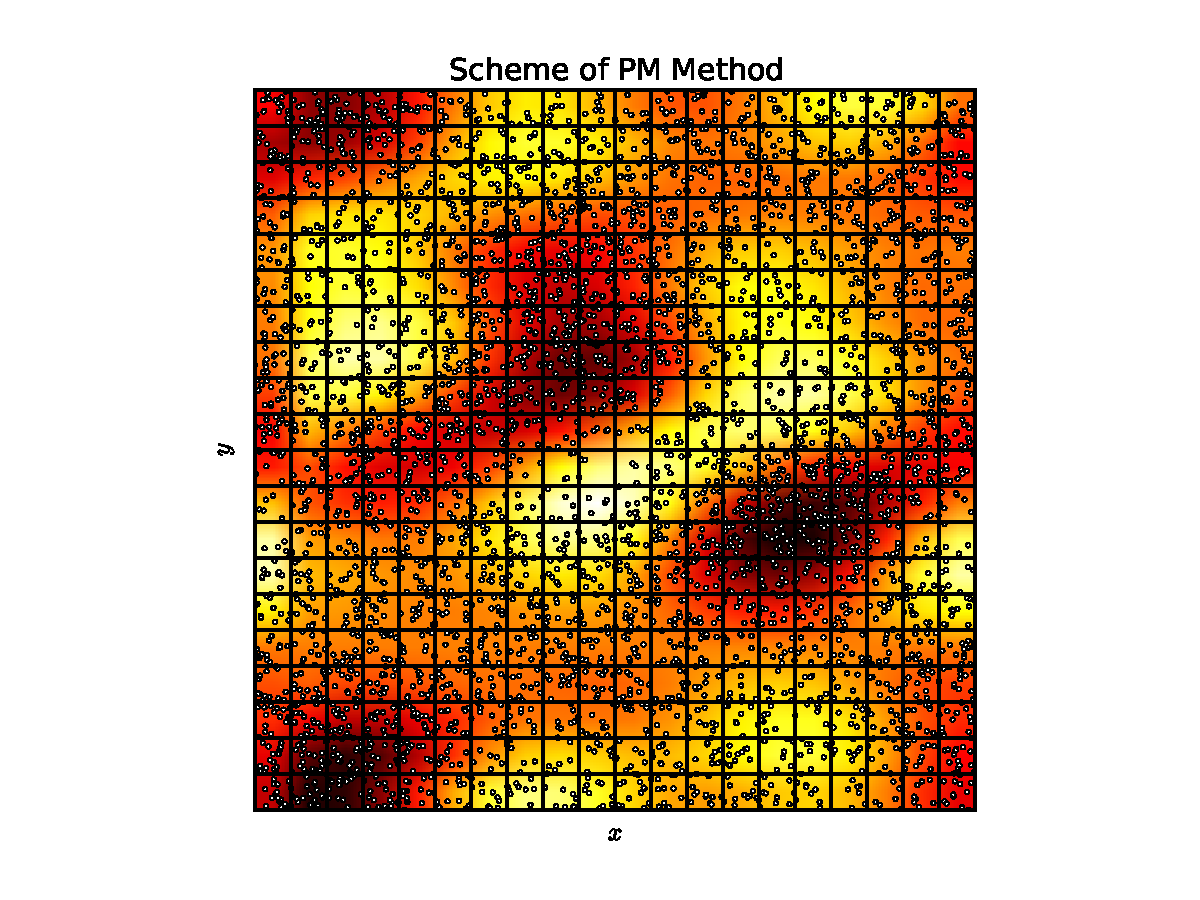
\includegraphics[width=1.00\textwidth]
	{./figures/3_nbody_simulations/PM_Method.pdf}

	\caption{\small{Illustrative diagram of the PM method. The map that is
	plotted over the distribution of particles corresponds to the density
	field evaluated in each cell of the grid. Dark cells corresponds to
	overdensity regions whereas white cells to lower values of the density 
	field, which agrees with the amount of mass of the particles per cell.}}
	
	\label{fig:MP_Method}
\end{figure}
%.........................................................................
%Reviewed
\newpage
The method can be summarized into the next steps


%Reviewed
%.........................................................................
%Particle Mesh steps
\begin{itemize}
\item[\textbf{1.}] From the grid established over all the simulation, it
is calculated a continuous density field $\rho(\bds r)$, interpolating the
value between adjacent cells.

%Reviewed
\item[\textbf{2.}] Once it is obtained the density field, it is calculated
the potential of the equation of movement \ref{eq:MovementEquation} by 
using the Poisson's equation



%.........................................................................
%Poisson Equation
\eq{eq:Poisson}
{ \nabla^2 \phi = 4 \pi G \rho }
%.........................................................................


%Reviewed
In order to reach this, it is usually used integration schemes based upon
Fourier transform, such as the Fast Fourier Transform (FFT).


%Reviewed
\item[\textbf{3.}] Finally, using the previous potential field, it is 
calculated the position of each particle in the next discrete time
$t+\Delta t$, and it is repeated over and over again until a given
final time.
\end{itemize}
%.........................................................................


%Reviewed
This method is less precise than the direct sum, but it is possible to 
demonstrate that the computing time scales as $t_{\submath{comp}} 
\propto N + M \log M$, with an asymptotic behaviour as $t_{\submath{comp}} 
\propto N$ for high resolutions $M$ of the grid and as $t_{\submath{comp}} 
\propto N$ for low resolutions \cite{pfalzner1996}. In any case, its 
efficiency is much better than the PP method \ref{subsec:PPMethod} when
the number of particles of the simulation is large enough $N\ll 10^4 - 
10^5$, which makes this method very useful to tackle problems with a large
number of particles.


%Reviewed
However, there are some pathological situations where this method can not
be applied satisfactory \cite{pfalzner1996}.


%Reviewed
%.........................................................................
%Difficulties of PM Method
\begin{itemize}
\item Highly non-homogeneous distributions of particles.
\item Strongly correlated systems.
\item Systems with non-trivial geometries.
\end{itemize}
%.........................................................................


%Reviewed
Because those conditions are satisfied in the non-linear universe, like 
strong gravitational couplings for modes of the density field after 
$z\gtrsim 8$, this methods is not very useful for solving the late 
universe.



	%---------------------------------------------------------------------
	%Hidrodynamical and dark matter simulations
	\subsection{P$^3$M Method}
	\label{subsec:P3Method}
	%---------------------------------------------------------------------
	
	
%Reviewed
The last of the three standard scheme for solving N-body simulations is 
the P$^3$M method (PP $+$ PM) \cite{hockney1988}. This method can be 
thought as a combination of the previous methods, making the most of each
one of them.


%Reviewed
%.........................................................................
%P3M Method
\begin{figure}[htbp]
	\centering
	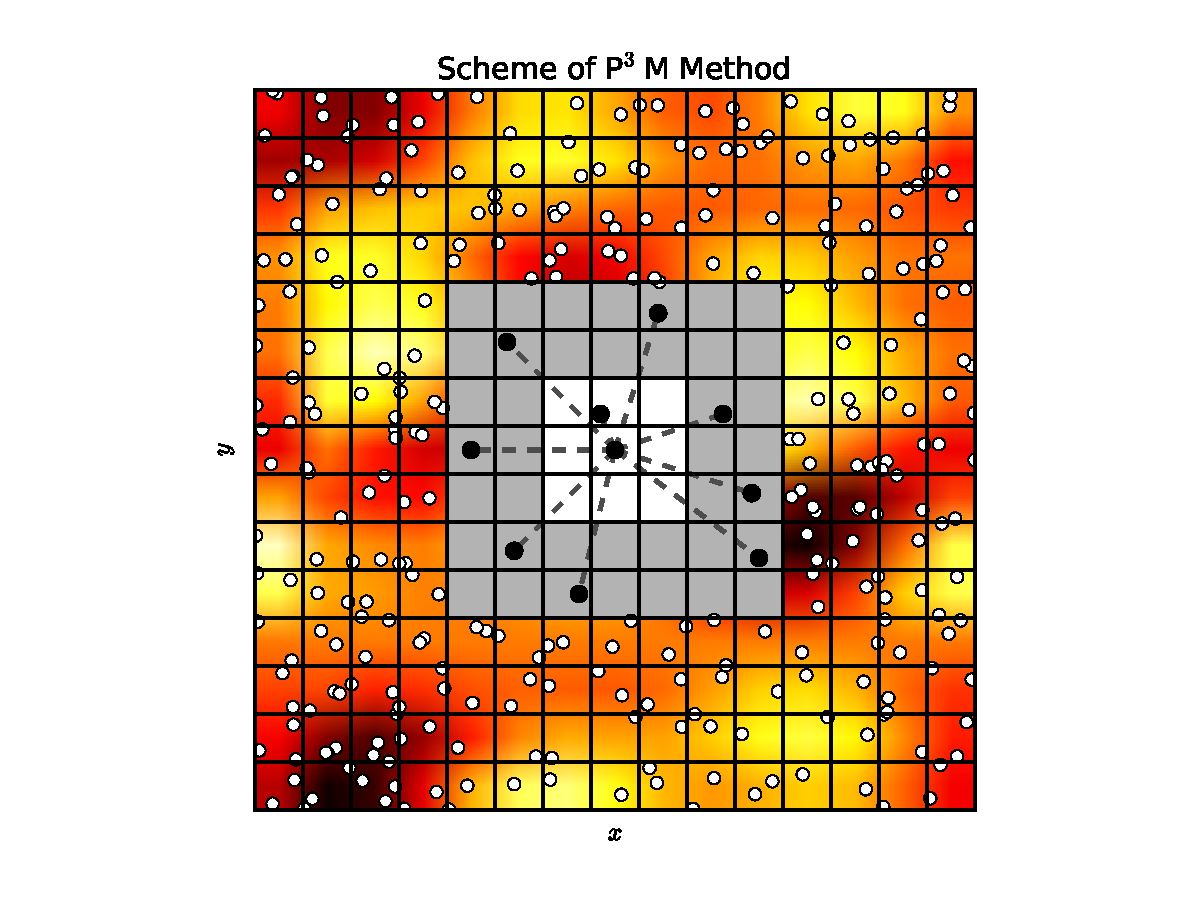
\includegraphics[width=1.00\textwidth]
	{./figures/3_nbody_simulations/P3M_Method.pdf}

	\caption{\small{Illustrative diagram of the P$^3$M method. For the 
	reference particle, shown in the center, interactions with distant 
	particles is calculated through the PM method, whereas for close
	particles (gray and white regions), the interaction is calculated 
	by using the PP method.}}
	
	\label{fig:P3M_Method}
\end{figure}
%.........................................................................


%Reviewed
Figure \ref{fig:P3M_Method} illustrates the P$^3$M method. For each one of
the integration step of the system, it is calculated a hierarchical grid 
for each particle. Hierarchies are defined with respect to the relative
distance between particles and they determines which approximation should
be used for computing the equation of movement. For close particles (first
hierarchy) it is used the PP method, what allows tackling strong local 
correlations and highly non-homogeneous regions. Interactions with 
particles embedded into the next hierarchies are calculated by decomposing 
the potential field into its multipolar terms, i.e. the second hierarchy
corresponds to the dipolar contribution of the potential (if applicable), 
and so on. Finally for more distant cells (last hierarchy), it is used the
PM scheme, interpolating the density field and solving the Poisson's 
equation \ref{eq:Poisson} for the potential.


%Reviewed
%.........................................................................
%Tree Code Building
\begin{figure}[htbp]
	\centering
	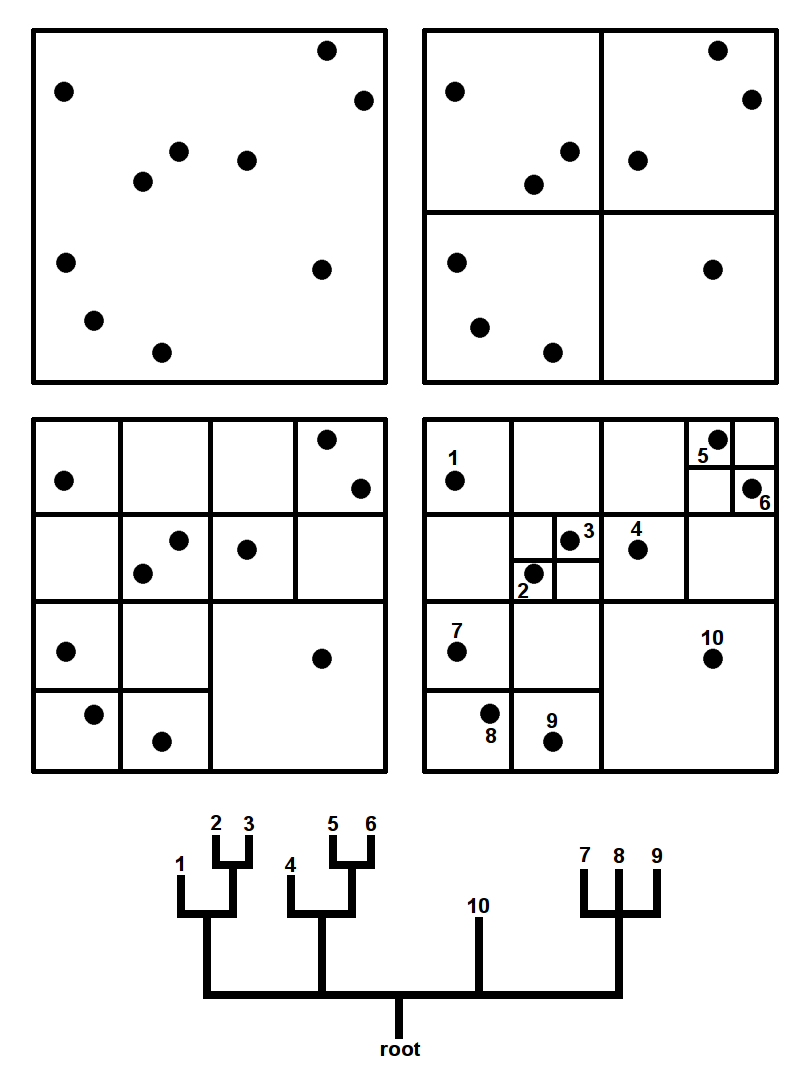
\includegraphics[width=0.72\textwidth]
	{./figures/3_nbody_simulations/TreeCode.png}

	\caption{\small{An illustrative example of the building of a tree code
	for a N-body simulation. Upper panels show the iterations for a 2D 
	problem whereas lower panel illustrates the resultant tree built using 
	each particle of the simulation.}}
	
	\label{fig:Tree_Code}
\end{figure}
%.........................................................................
\newpage


%Reviewed
One of the main disadvantages of this method lies in the building of the
hierarchical structure for evaluating which scheme must be used. The 
original scheme proposed simultaneously by \cite{appel1985} 
\cite{jernigan1985} and \cite{porter1985} has some inconsistencies 
produced by the lack of physical basis in the building of the hierarchical
structure \cite{pfalzner1996}.


%Reviewed
A better physically based method for constructing the hierarchical 
structure of a N-body simulation is the so-called octant tree code. It was
initially developed by \cite{barnes1986}. In this algorithm, the space of 
the simulation is embedded into a cubic volume denominated \textit{root},
then this volume is divided into 8 regions of equal size which are 
denominated octant, these are the first hierarchy of the tree. This 
procedure is repeated recursively until each cell or octant has only one
particle inside, thereby constructing a set of hierarchies that determines
the neighbourhood of all the particles of the simulation. Figure 
\ref{fig:Tree_Code} illustrates the iterations needed in order to construct
the tree of a simulation (with the aim of simplicity, it is 2D), the lower
panel of the same figure shows the structure of the tree. In this way it
is possible to compute, for instance, the interaction between particles 7,
8 and 9 by using direct sum, because they are the closer neighbours, 
whereas the interaction with other particles that belong to other branches
is calculated through the PM scheme.



%*************************************************************************




%*************************************************************************
%Types of simulations
\section{Tipos de Simulación}
\label{sec:Types of Simulations}


Usando los métodos descritos en la anterior subsección es posible realizar
simulaciones del universo en régimen no lineal y estudiar su comportamiento 
de forma numérica. Debido a que en régimen no lineal los procesos 
astrofísicos de grandes escalas son dominados principalmente por materia 
oscura, es habitual no consi\-derar la contribución de las componentes de 
radiación y materia bariónica, además de que los procesos físicos que 
involucran estás componentes aumentarían conside\-rablemente los tiempos 
de cómputo. Este tipo de simulaciones son denominadas \textit{simulaciones 
de materia oscura}.


En esta subsección son presentadas las simulaciones de materia oscura que 
son usadas, además son clasificadas acorde al criterio adoptado para la 
elección de las condiciones iniciales. Estas pueden ser no restringidas
cuando las condiciones iniciales son escogidas de forma completamente 
aleatoria, o restringidas cuando son escogidas de tal forma que la 
simulación satisfaga alguna condición impuesta a priori, tal como la 
reproducción del universo local en una escala de algunas decenas de 
Mpc$/h$.


	%---------------------------------------------------------------------
	%Unconstrained simulations (Bolshoi)
	\subsection{Simulaciones No Restringidas (Bolshoi)}
	\label{subsec:UnconstrainedSimulations}
	%---------------------------------------------------------------------


Puesto que la evolución del universo en régimen lineal es conocida a 
través de la función de transferencia (ver sección 
\ref{sec:LinearStructureFormation}), las simulaciones cosmológicas solo 
son usadas para el estudio del régimen no lineal, aún así es necesario
fijar un conjunto de condiciones iniciales para la integración del sistema.
Generalmente estas condiciones son determinadas a partir del cómputo del 
régimen lineal, para esto a su vez es requerido otro conjunto de condiciones 
iniciales primordiales para el campo de densidad homogéneo de fondo, 
es debido a esto que estas últimas condiciones serán referidas simplemente 
como condiciones iniciales.


Como ha sido mencionado en la subsección \ref{subsec:StatisticalProperties},
las propiedades estadísticas del campo de densidad inicial corresponden a 
una distribución Gaussiana de los modos de Fourier con un espectro de
potencia de Harrison-Zeldovich, acorde con el modelo inflacionario y 
observaciones cosmológicas (subsección \ref{sec:CosmologicalObservations}).
Los modos del campo de densidad $\delta_{\bds k} = 
r_{\bds k}e^{i\phi_{\bds k}}$ siguen entonces las distribuciones 
determinadas en la ecuación \ref{eq:GaussianDistribution}


%.........................................................................
%Radial distribution
\eq{eq:RadialModeDistribution}
{ P_r(r_{\bds k})dr_{\bds k} = \exp\pr{ -\frac{r_{\bds k}^2}{\sigma_k^2} }
\frac{2r_{\bds k}dr_{\bds k}}{\sigma_k^2} }
%.........................................................................


%.........................................................................
%Angular distribution
\eq{eq:PhiModeDistribution}
{ P_\phi(\phi_{\bds k})d\phi_{\bds k} = \pr{\frac{1}{2\pi}}d\phi_{\bds k} }
%.........................................................................


El carácter no restringido de este tipo de simulaciones radica en la 
elección aleatoria de las fases $\phi_{\bds k}$ acorde a la distribución
\ref{eq:PhiModeDistribution}, sin ningún tipo de restricción observacional
sobre el resultado final de la simulación.

\

\textbf{\textit{Bolshoi}} es una simulación cosmológica del universo 
a gran escala con condiciones iniciales no restringidas, la página 
oficial del proyecto es \url{http://hipacc.ucsc.edu/Bolshoi/}. 

\newpage
%.........................................................................
%Bolshoi Simulation Evolution
\begin{figure}[htbp]
	\centering
	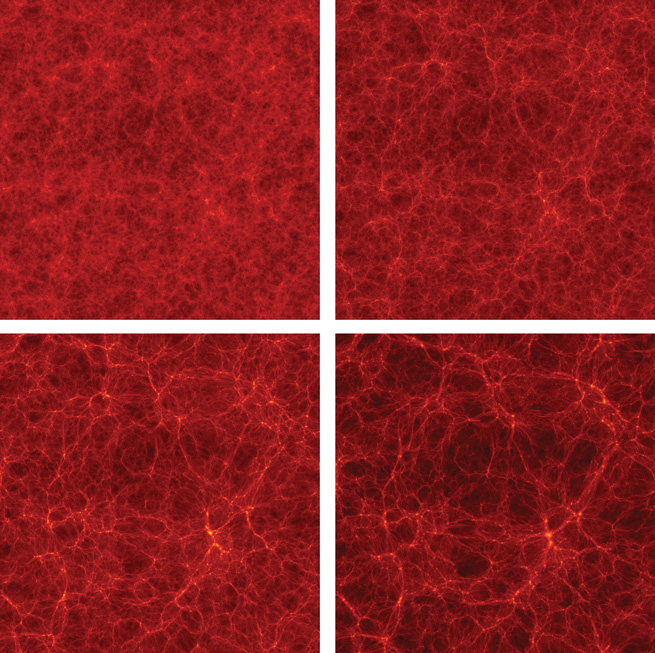
\includegraphics[width=0.85\textwidth]
	{./figures/3_nbody_simulations/Bolshoi_Evolution.png}

	\caption{\small{Evolución de la simulación Bolshoi. Se ilustran el
	campo de densidad de una región rectangular de 16 Mpc$/h$ de grosor y 
	250 Mpc$/h$	de lado para diferentes estadios de evolución. $z=9.5$ 
	(superior izquierda), $z=3$ (superior derecha), $z=1$ (inferior 
	izquierda) y $z=0$ (inferior derecha). Tomado de 
	\url{http://spectrum.ieee.org/aerospace/astrophysics/the-cosmological-supercomputer} }}
	
	\label{fig:Bolshoi_Evolution}
\end{figure}
%.........................................................................


Debido a su mayor tamaño comóvil comparada con las simulaciones 
restringidas (un cubo de $250$ Mpc$/h$ de lado), esta es usada para 
obtener estadística más fina en los resultados del capítulo 
\ref{cha:Results}. El modelo cosmológico usado para esta simulación 
corresponde al WMAP7 (ver tabla \ref{tab:CosmologicalParameters}), el número 
de partículas es de $2048^3$, lo que implica una masa promedio por partícula 
de $1.35 \times 10^8 h^{-1}$ M$_{\odot}$. Una descripción técnica más 
detallada de la simulación puede ser consultada en \cite{klypin2011}.
\newpage

	%---------------------------------------------------------------------
	%Constrained simulations (CLUES)
	\subsection{Simulaciones Restringidas (CLUES)}
	\label{subsec:ConstrainedSimulations}
	%---------------------------------------------------------------------


Como fue mencionado en el capítulo \ref{cha:Theoretical Framework}, la forma
estándar de comparar el resultado de simulaciones cosmológicas con 
observaciones es a través de las propiedades estadísticas de las 
distribuciones, tales como funciones de correlación de dos puntos o 
espectros de potencia. A pesar de esto, algunos estudios requieren una 
descripción detalla del universo local en un contexto cosmológico. Debido 
a dificultades técnicas como la medida directa de la distribución de materia
oscura o la falta de datos en altos corrimientos al rojo, es necesario 
recurrir a simulaciones cosmológicas que reproduzcan el universo local.
Uno de los primeros trabajos dirigidos a la reproducción específica del
entorno local se debe a \cite{Klypin2003}. En este se intenta reproducir las 
principales estructuras observadas en el universo local, como el grupo local,
el Supercúmulo Local y el cúmulo de Virgo.


%.........................................................................
%Constrained Simulation
\begin{figure}[htbp]
	\centering
	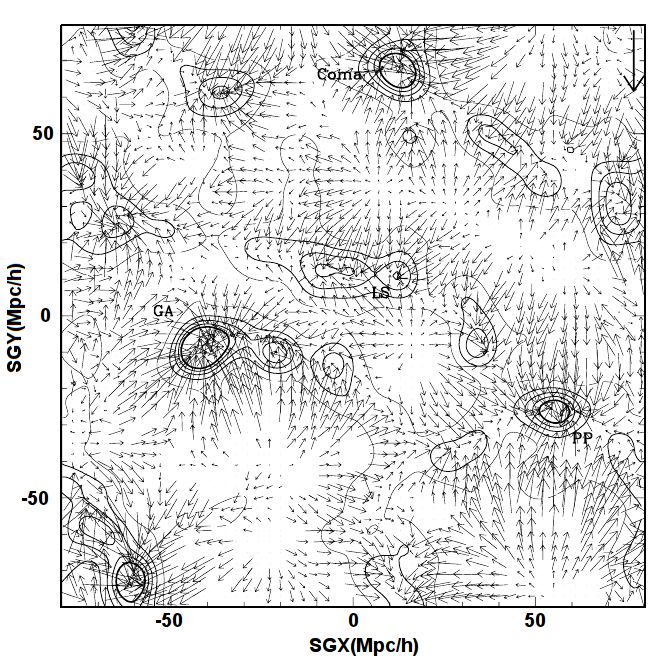
\includegraphics[width=0.60\textwidth]
	{./figures/3_nbody_simulations/Constrained_Construction.png}

	\caption{\small{Campo de densidad y campo de velocidad peculiar inicial
	construidos a partir de restricciones para la reproducción del entorno
	local en una escala de $160\ h^{-1}$Mpc. Algunas estructuras 
	identificadas son: \textit{Coma}, cúmulo de coma, \textit{PP}, supercúmulo 
	de Perseus-Pisces, \textit{LS}, supercúmulo local, \textit{GA}, gran 
	atractor. La flecha superior derecha indica la escala del campo de 
	velocidad peculiar en $1000$ km/s. Tomado de \cite{Klypin2003}.}}
	
	\label{fig:Constrained_Construction}
\end{figure}
%.........................................................................


El método propuesto en \cite{Klypin2003} y \cite{Hoffman1991} consiste en 
la construcción el campo de densidad y de velocidad peculiar inicial a 
partir de surveys de velocidades radiales y de corri\-mientos al rojo (ver 
sección \ref{sec:CosmologicalObservations}). Para el tratamiento y 
reducción del ruido y errores de medida en los datos, se usa un método 
bayesiano de filtros de Wiener (para más detalles técnicos ver 
\cite{Zaroubi1999}). A pequeñas escalas este método es limitado debido a 
que los filtros aplicados suprimen algunos modos en el espectro de potencia 
inicial y por tanto deben ser generados de forma aleatoria acorde con la 
distribución Gaussiana \ref{eq:GaussianDistribution} para garantizar 
consistencia con el modelo cosmológico estándar. En la figura 
\ref{fig:Constrained_Construction} se ilustran las condiciones iniciales 
obtenidas con este método para el universo local en una escala de 
$160\ h^{-1}$Mpc.


%.........................................................................
%CLUES Right Simulation
\begin{figure}[htbp]
	\centering
	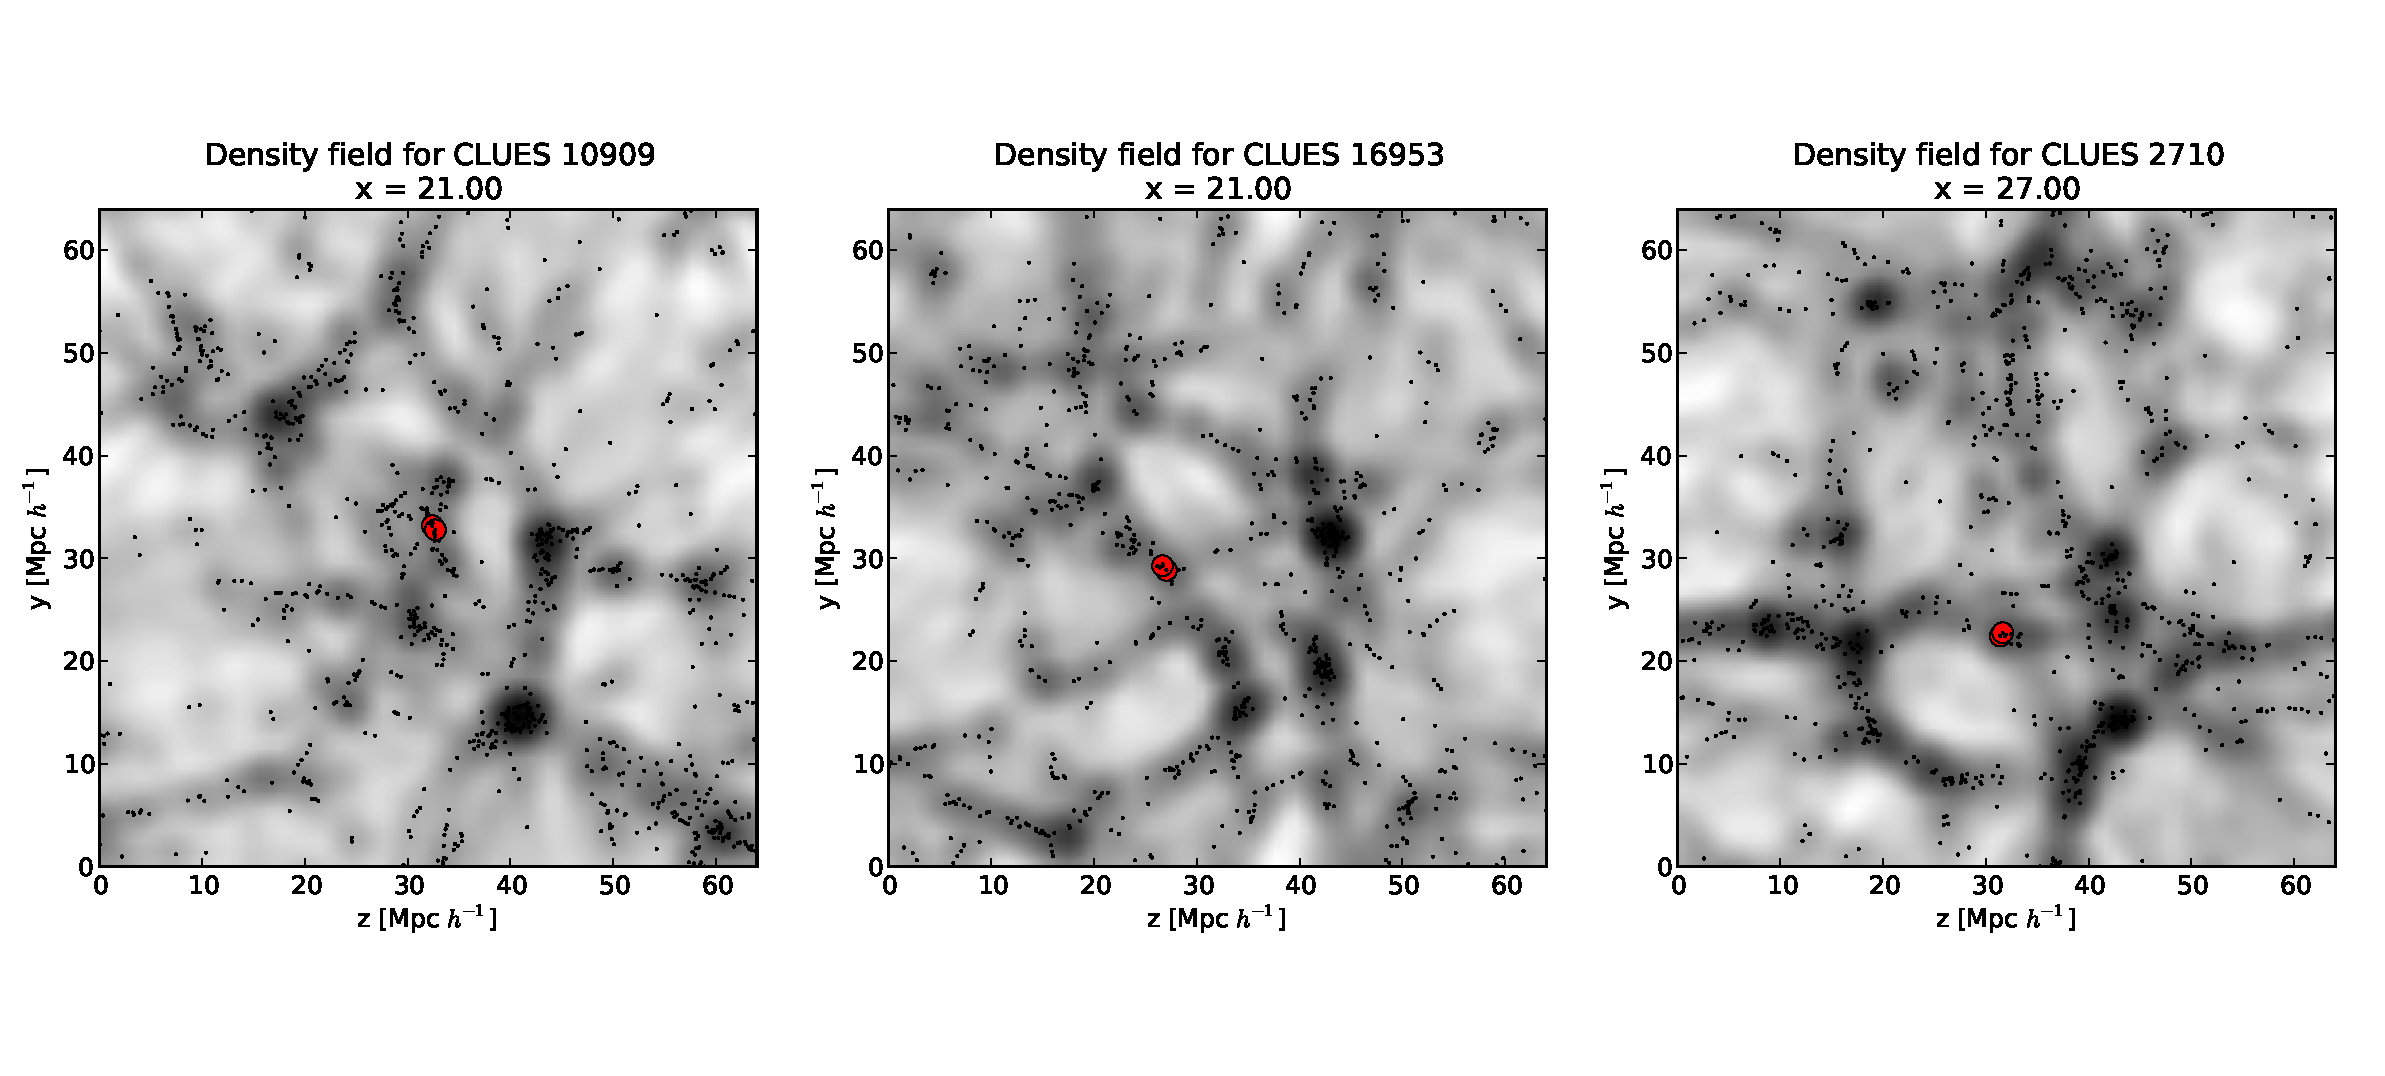
\includegraphics[width=1.0\textwidth]
	{./figures/3_nbody_simulations/CLUES_Simulations.pdf}

	\caption{\small{Tres simulaciones restringidas del proyecto CLUES 
	en las se identifican sistemas tipo grupo local. Se ilustra el campo 
	de densidad de cada simulación junto con los halos de materia oscura
	(puntos negros), y los grupos locales encontrados (puntos rojos).}}
	
	\label{fig:CLUES_Right}
\end{figure}
%.........................................................................


\textbf{CLUES} (Constrained Local UniversE Simulations) es un proyecto 
orientado a la reproducción del universo local con la mejor resolución 
en la actualidad. La página oficial es \url{http://www.clues-project.org}. 
En estas simulaciones las condiciones iniciales son construidas con el 
algoritmo Hoffman-Ribak \cite{Hoffman1991} para la reproducción de un 
volumen comóvil de $(64\ h^{-1}$Mpc$)^{3}$. Debido a la no restricción en
escalas pequeñas ($\sim 5\ h^{-1}$Mpc) es necesario realizar $200$ 
diferentes simulaciones de las cuales $3$ resultan satisfactorias 
respecto a las restricciones observacionales (ver figura 
\ref{fig:CLUES_Right}). Para la evolución se usa el paquete 
\texttt{GADGET2}\footnote{\texttt{GADGET2} es un popular código para la 
simulación de N-cuerpos en cosmología y formación de galaxias. Está 
disponible de forma gratuita en la página oficial del proyecto 
\url{http://www.mpa-garching.mpg.de/gadget/}} con $1024^3$ partículas de
materia oscura y una cosmología consistente con el WMAP7 (ver tabla 
\ref{tab:CosmologicalParameters}). Más detalles técnicos del proyecto
pueden ser consultados en \cite{Gottloeber2010}.


%.........................................................................
%CLUES Simulation Overview
\begin{figure}[htbp]
	\centering
	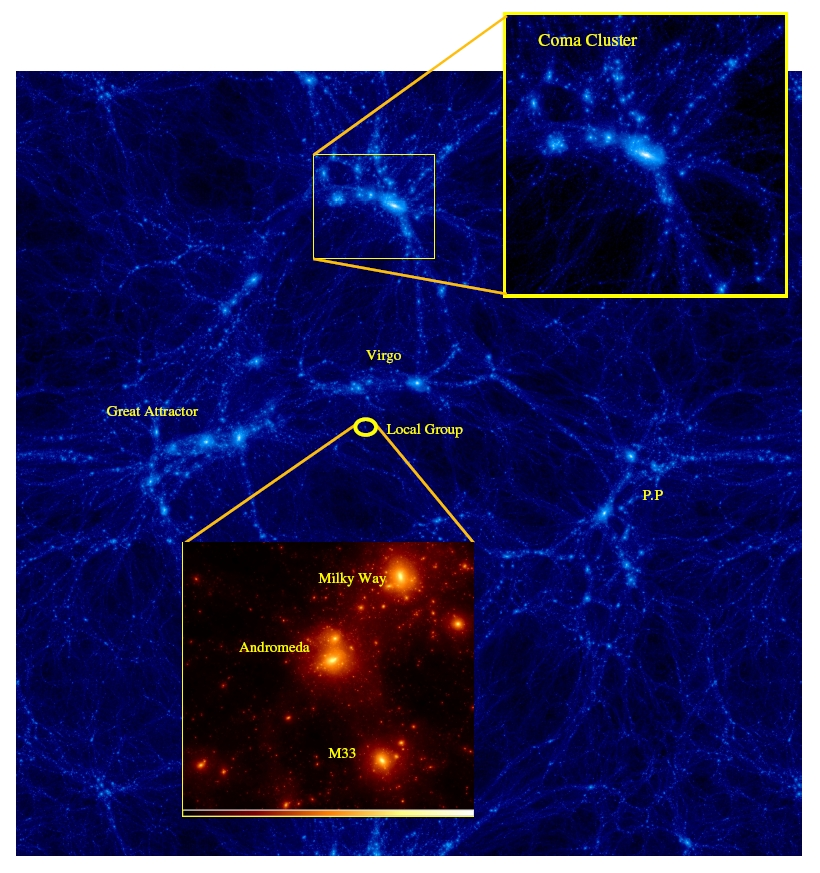
\includegraphics[width=0.90\textwidth]
	{./figures/3_nbody_simulations/CLUES_Overview.png}

	\caption{\small{Simulación obtenida en el proyecto CLUES. En esta se 
	muestran las estructuras a gran escala del universo local y se aprecian
	con claridad los miembros más significativos del grupo local. Tomado de 
	la 	página oficial del proyecto \url{http://www.clues-project.org}}}
	
	\label{fig:CLUES_Overview}
\end{figure}
%.........................................................................


%*************************************************************************



%*************************************************************************
%Environment Characterization
\section{Caracterización del Entorno}
\label{sec:EnvironmentCharacterization}


Una vez obtenidas las simulaciones numéricas de la evolución en régimen no 
lineal, uno de los principales objetivos es caracterizar las estructuras 
emergentes propias de este régimen. Entre estas destaca la gran estructura 
de red que se forma a partir de regiones de diferente dimensionalidad, 
donde grandes regiones vacías son limitadas por regiones planas, estas a 
su vez son recorridas por filamentos unidimensionales que se juntan en regiones 
puntuales altamente densas (red cósmica). 


A partir de observaciones cosmológicas se ha logrado establecer la 
relación entre las propiedades de halos de galaxias, tales como el parámetro 
de espín, la concentración, la forma, etc. Y el entorno donde están 
embebidas. Debido a esto es importante cuantificar la estructura de red 
cósmica en simulaciones cosmológicas. Uno de los primero trabajos en esta 
dirección consiste en la aproximación de Zeldovich mostrada en la subsección 
\ref{subsec:Zeldovich'sApproximation}), otros esquemas posteriores usan 
estratificaciones del campo de densidad para cuantificar el entorno y son 
denominados métodos geométricos, pero debido a su carácter local no 
pueden dar cuenta de propiedades más globales como canales de flujo de 
materia o influencia de grandes estructuras cercanas. En esta sección se 
muestran dos esquemas para la clasificación del entorno desarrollados 
recientemente.


	%---------------------------------------------------------------------
	%The T-web Method
	\subsection{Método T-web}
	\label{subsec:TheT-webMethod}
	%---------------------------------------------------------------------


El primero de los métodos fue propuesto por \cite{Hahn2007} y consiste el
uso de la teoría de sistemas dinámicos para el análisis de la estabilidad 
local de órbitas de prueba alrededor de halos de materia oscura y de esta 
forma cuantificar su entorno para un tiempo (corrimiento al rojo) fijo 
dado. Para esto se asume válida la aproximación Newtoniana (ver subsección 
\ref{subsec:Newtonian Approximation}) y la ecuación de movimiento de una 
partícula de prueba en el potencial peculiar de la distribución es


%.........................................................................
%Equation of Movement 
\eq{eq:Tweb_Movement}
{ \ddot{\bds r} = - \nabla \phi(\bds r) \ \ \ \ 
\mbox{con}\ \ \ \ \ \nabla^2 \phi = 4\pi G \bar \rho \delta}
%.........................................................................


Es razonable asumir que en el centro de masa $\bar{\bds r}_i$ de cada halo
existe un mínimo del potencial $\nabla \phi = 0$, formando así un pozo de 
potencial local. Esto permite linea\-lizar la ecuación de movimiento 
\ref{eq:Tweb_Movement} entorno a estos puntos, obteniendo


%.........................................................................
%Lineal Equation of Movement 
\eq{eq:Lineal_Tweb}
{ \ddot{r}_i = - T_{ij}(\bar{\bds r}_i)( r_j - \bar{ r}_{k,j})}
%.........................................................................
donde se define el tensor de marea como el Hessiano del potencial peculiar


%.........................................................................
%Tweb Tensor
\eq{eq:Tweb_Definition}
{ T_{ij} \equiv \frac{\partial^2 \phi}{\partial r_i \partial r_j}}
%.........................................................................


Acorde a la teoría de sistemas dinámicos, un autovalor negativo indica que
el punto es inestable en la dirección del respectivo autovector, implicando 
un flujo de materia hacia el exterior de la región. Para autovalores 
positivos se presenta una situación completamente análoga. Con base en la 
aproximación de Zeldovich (subsección \ref{subsec:Zeldovich'sApproximation})
se propone un esquema de clasificación del entorno cosmológico a partir de 
los autovalores del tensor de marea $T_{ij}$ 
(ver figura \ref{fig:ClassificationSchemeTweb}).


%.........................................................................
%Classification of Cosmological Environment
\begin{itemize}
\item \textbf{Vacío (Vacuum):} en este caso los tres autovalores son positivos, 
indicando una expansión en todas las direcciones.
\item \textbf{Hoja (Sheet):} para este caso $\lambda_1\geq\lambda_2>0$ y 
$\lambda_3<0$, indicando un colapso en una sola dirección, dando lugar a una 
zona con geometría local plana.
\item \textbf{Filamento (Filament):} para estas zonas solo el $\lambda_1$ es
positivo, indicando un colapso en dos direcciones y expansión e una, formando
así una región con geometría unidimensional.
\item \textbf{Nudo (Knot):} para este último tipo de región, los tres 
autovalores son negativos, indicando un colapso en todas las direcciones y 
dando lugar a una zona comprimida.
\end{itemize}
%.........................................................................


Lo más destacable de este método respecto a los métodos geométricos es su 
naturaleza dinámica, permitiendo diferenciar zonas con iguales valores 
densidad pero con propiedades de estabilidad diferentes. A pesar de lo 
anterior, la asunción de mínimo local solo es justificada en el centro de 
cada halo, careciendo así de significado y precisión generalizar este 
esquema en cualquier punto del espacio. Otro inconveniente es que bajo el 
esquema de clasificación original con los signos de cada autovalor no se 
reproduce la impresión visual que se obtiene en la distribución de materia
de las simulaciones (ver figura \ref{fig:TwebVwebComparison}).


%.........................................................................
%Classification Scheme
\begin{figure}[htbp]
	\centering
	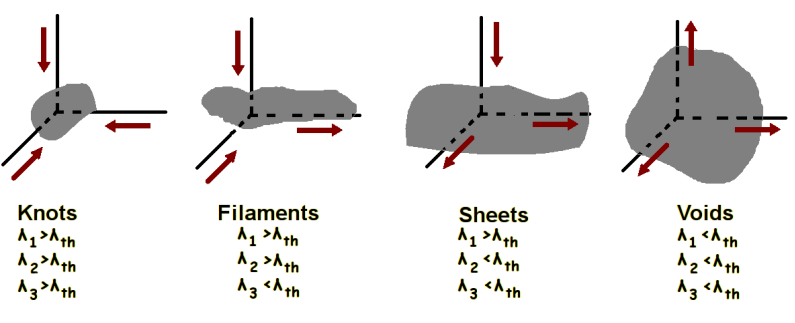
\includegraphics[width=0.9\textwidth]
	{./figures/2_theoretical_framework/EnvironmentClassification.png}

	\caption{\small{Esquema de clasificación del entorno cosmológico 
	para los esquemas T-web y V-web. El valor umbral $\lambda_{th}$ es 
	tomado como un parámetro libre.}}
	
	\label{fig:ClassificationSchemeTweb}
\end{figure}
%.........................................................................


Una significativa mejora de este método se logra generalizando el esquema 
de clasificación respecto a un cierto valor umbral $\lambda_{th}^T$, que 
es tomado como parámetro libre y se ajusta acorde a la impresión visual 
obtenida \cite{forero2008}, en especial el esquema original se recupera 
fijando $\lambda_{th}^T=0$.


	%---------------------------------------------------------------------
	%The V-web Method
	\subsection{Método V-web}
	\label{subsec:TheV-webMethod}
	%---------------------------------------------------------------------


El segundo método dinámico presentado para la clasificación de la red 
cósmica es presentado en \cite{hoffman2012} y está basado en el tensor de 
velocidad de peculiar (shear velocity tensor)


%.........................................................................
%Vweb Tensor
\eq{eq:Vweb_Definition}
{ \Sigma_{ij} = -\frac{1}{2 H_0}\pr{ \der{v_i}{r_j} + \der{v_j}{r_i} } }
%.........................................................................
de forma análoga al esquema T-web, en este esquema son calculados los 
auto\-valores del tensor $\Sigma_{ij}$ y se define el entorno acorde a un 
valor umbral $\lambda_{th}^V$ (ver figura \ref{fig:ClassificationSchemeTweb}).


Como es mostrado en \cite{hoffman2012}, en el régimen lineal los tensores
$T_{ij}$ y $\Sigma_{ij}$ son proporcionales, siendo ambos métodos 
completamente equivalentes en este régimen. Esto es parcialmente 
evidenciado en la impresión visual de ambos esquemas de clasificación que 
se obtiene a grandes escalas para la simulación Bolshoi (figura 
\ref{fig:TwebVwebComparison}), y se debe a la menor no linealidad de los 
modos a mayores escalas. 


%.........................................................................
%Tweb Vweb Comparison
\begin{figure}[htbp]
	\begin{center}
	\makebox[\textwidth]{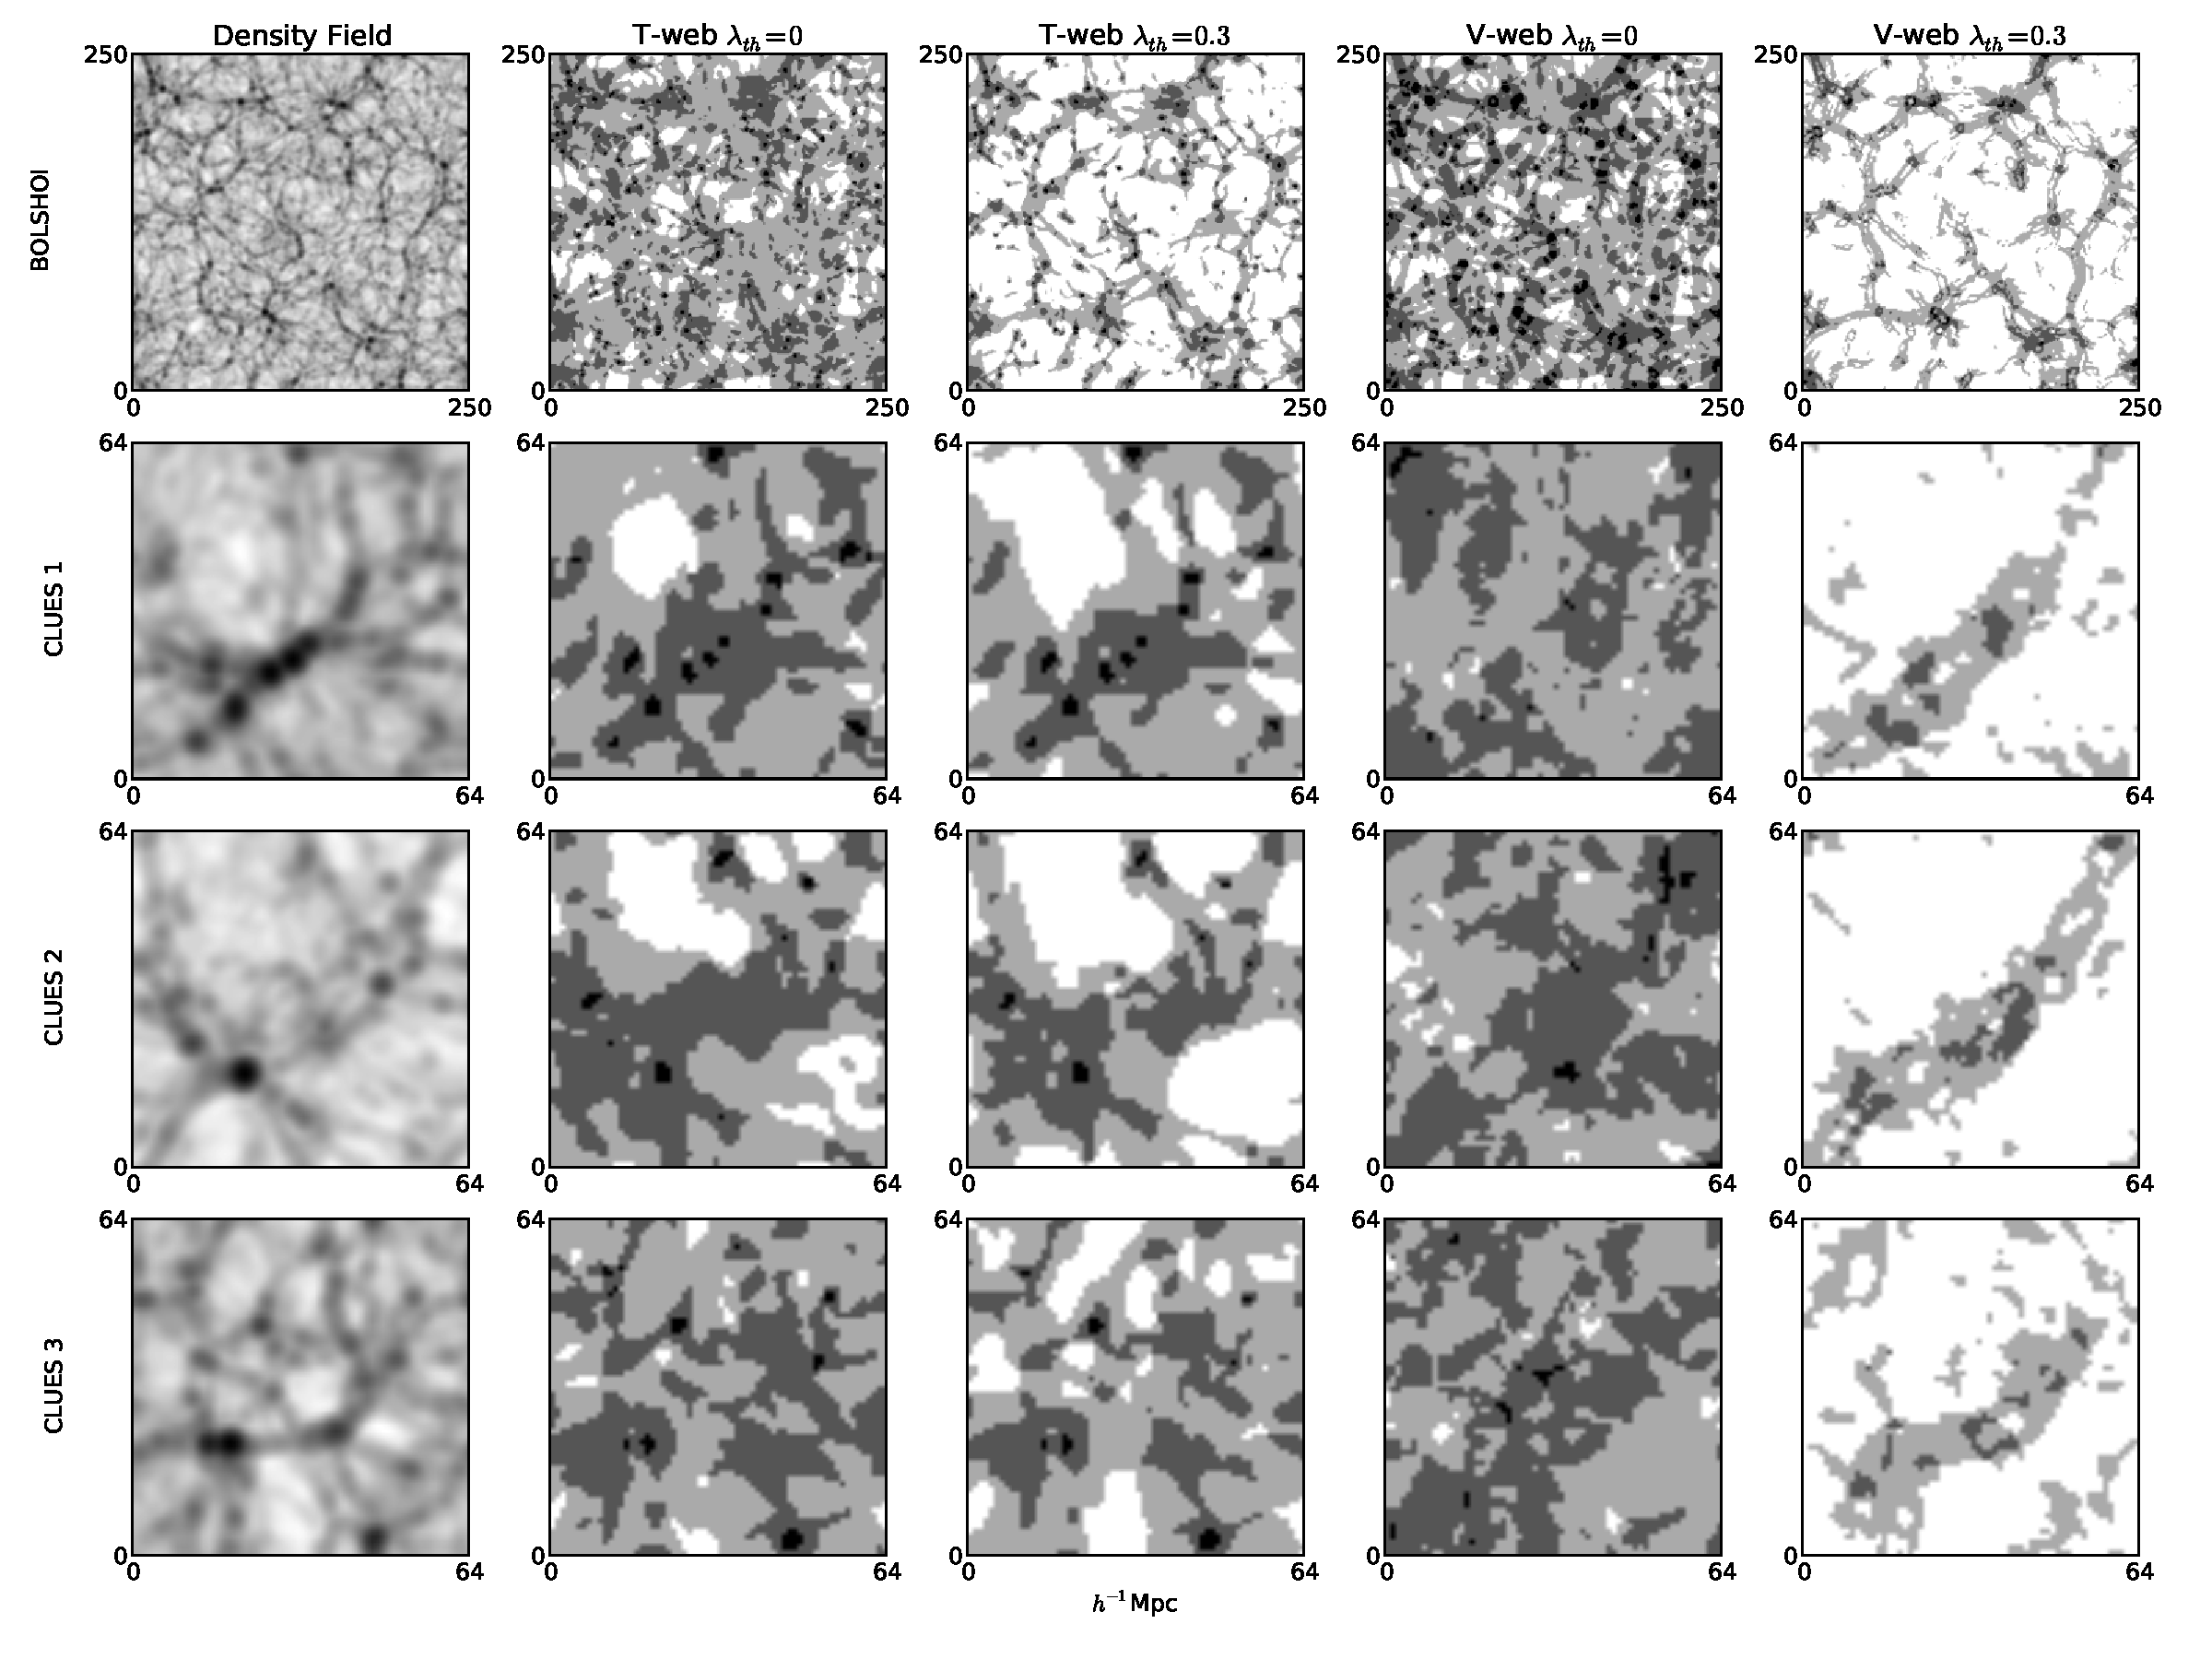
\includegraphics[trim = 5mm 8mm 10mm 5mm, clip, 
	width=0.80\paperwidth,angle=-90]
	{./figures/3_nbody_simulations/Vweb_Tweb.pdf}}
	\end{center}

	\caption{\small{Se ilustra para cada una las simulaciones
	(CLUES 1, CLUES 2, CLUES 3, Bolshoi) la diferencia entre los 
	esquemas de clasificación T-web y V-web para diferentes valores de 
	$\lambda_{th}$ (Negro - Nudo, Gris oscuro - Filamento, Gris - Hoja, 
	Blanco - Vacío). En las gráficas superiores se muestra la impresión 
	visual obtenida a partir de los respectivos campos de contraste de 
	densidad ($\log (\delta+1)$), usadas para la calibración de los valores 
	$\lambda_{th}$. La resolución para una de las mallas construidas es 
	aproximadamente $1.0 h^{-1}$ Mpc/celda y para todas se realiza un
	suavizado Gaussiano del tamaño de una celda, el grosor de cada slide
	es de una celda de la malla.}}
	
	\label{fig:TwebVwebComparison}
\end{figure}
%.........................................................................


En el caso de modos pequeños, donde los efectos no lineales son más 
do\-minantes, ambos esquemas difieren notablemente, tal como puede verse en 
la impresión visual de las simulaciones CLUES. Específicamente, el esquema 
V-web cuantifica de forma más precisa la estructura fina de la red 
cósmica a pequeñas escalas, permitiendo definir un entorno más apropiado 
para pequeñas estructuras a nivel cosmológico como halos de materia oscura 
o pequeños grupos de ellos.


Otra ventaja del esquema V-web respecto al T-web radica en que está basado 
en el campo de velocidades peculiares en vez del campo de densidad, aportando 
así más información dinámica del entorno y haciendo posible dar cuenta de una
forma más directa de efectos no locales, como flujos de materia o influencia 
de estructuras cercanas. Debido a esto, este esquema será adoptado como 
estándar para la cuantificación del entorno de halos y pares de halos 
(sistemas como el grupo local) y de las distribuciones de entorno 
cosmológico en el capítulo \ref{cha:Results}.


%*************************************************************************




%*************************************************************************
%Halos detection and sample definitions
\section{Detección de Halos y Definición de Muestras}
\label{sec:HalosDetectionAndSampleDefinitions}


Una vez caracterizado el entorno cosmológico, el siguiente paso es encontrar 
las estructuras que se forman en las simulaciones, específicamente halos de 
materia oscura. Debido a la naturaleza continua de la distribución de materia 
en el universo, es complicado y subjetivo definir estructuras discretas y 
limitadas espacialmente, como los halos de materia oscura o las galaxias en 
ellos. A pesar de esto, el carácter aproximado de las soluciones numéricas 
exige a priori uan construcción discreta del campo de densidad a partir de 
partículas puntuales con una cierta masa representativa (generalmente del 
orden de $10^7 \sim 10^9 h^{-1}$ M$_{\odot}$, aunque depende específicamente 
de la resolución de la simulación), esto implica que la detección de 
estructuras físicas discretas\footnote{A pesar de que las partículas que 
mapean la distribución de densidad también tienen un carácter discreto, su 
individualidad carece de sentido físico y solo es consecuencia de los 
métodos numéricos implementados.} se reduce a encontrar agrupaciones de 
partículas que representen estos sistemas.


	%---------------------------------------------------------------------
	%FOF method
	\subsection{Método FOF}
	\label{subsec:FOFMethod}
	%---------------------------------------------------------------------
	

Uno de los métodos más utilizados para la detección de estructuras en 
simulaciones de N-cuerpos se denomina FOF (por sus siglas en inglés
\textit{Friend of Friend}).

\
%.........................................................................
%FOF Method
\begin{figure}[htbp]
	\centering
	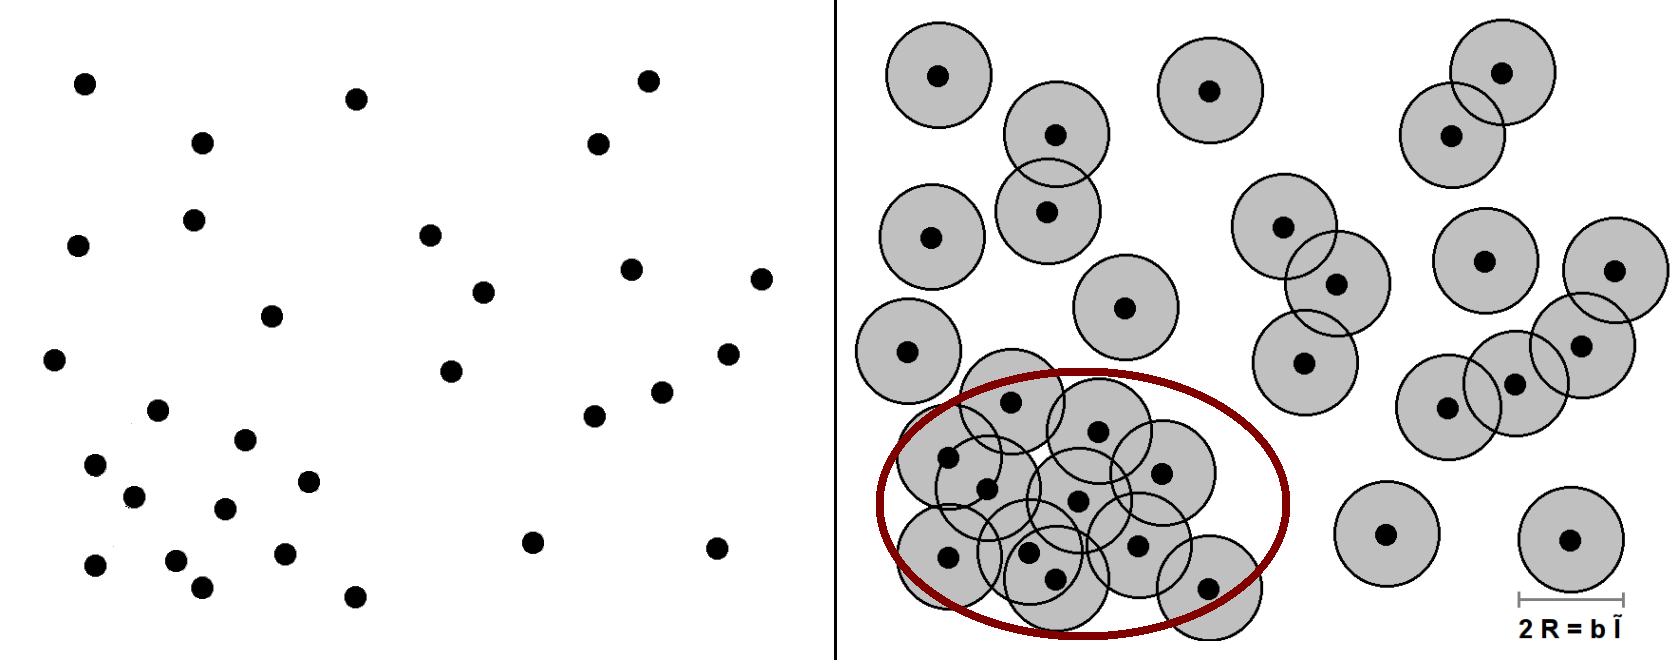
\includegraphics[width=0.9\textwidth]
	{./figures/3_nbody_simulations/FOF_Method.png}

	\caption{\small{Diagrama ilustrativo del método FOF. Los círculos grises
	entorno a cada partícula representa la zona de vinculación y la curva 
	roja representa una de las estructuras encontradas.}}
	
	\label{fig:FOF_Method}
\end{figure}
%.........................................................................


En este método se asocia un volumen finito a cada partícula, denominada 
región de vinculación, luego las estructuras son halladas a partir de 
intersecciones contiguas de estas regiones. Un ejemplo ilustrativo es 
presentado en la figura \ref{fig:FOF_Method}, donde la estructura de la curva
roja, correspondiente a un halo de materia oscura, es construida a partir
de 11 regiones de vinculación adyacentes que se intersectan mutuamente.
La geometría de las regiones de vinculación son generalmente esféricas, con
un radio $R_i$ dado por la siguiente expresión


%.........................................................................
%FOF Diameter
\eq{eq:FOF_Diameter}
{ R_i = \frac{1}{2}b\ \bar l }
%.........................................................................
donde $b$ es el parámetro de vinculación y $\bar l$ el camino libre medio 
de las partículas en la simulación. El parámetro de vinculación $b$ es libre 
y depende de cada simulación, siendo especificado a priori en la construcción 
de catálogos de halos.


En la figura \ref{fig:CLUES_FOF} se muestra el resultado del método FOF en
la construcción de un catálogo de halos de materia oscura para la simulación
CLUES 3. La distribución de los halos está acorde con la distribución de 
densidad (ver figura \ref{fig:TwebVwebComparison}), siguiendo el mismo patrón
de filamentos y nodos de la red cósmica. En el subsección 
\ref{subsec:SampleOfPairsToUse}, las muestras de halos definidas en cada 
simulación se hallan a partir de este esquema, con un parámetro de 
vinculación $b = 0.17$.


%.........................................................................
%FOF method in CLUES simulation
\begin{figure}[htbp]
	\centering
	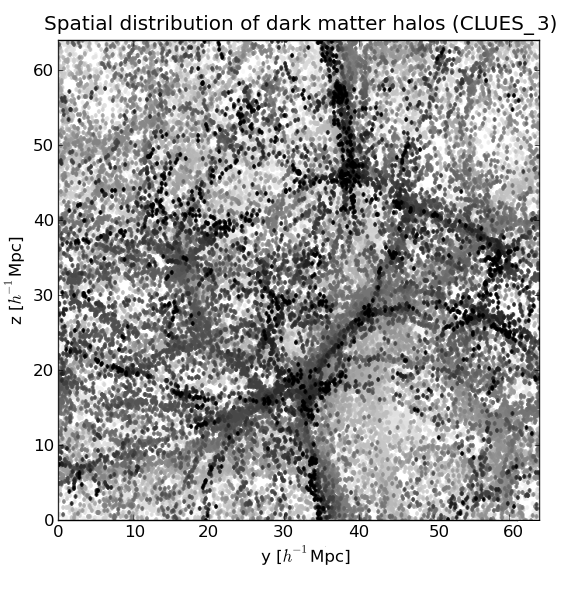
\includegraphics[width=0.5\textwidth]
	{./figures/3_nbody_simulations/Halos_Spatial_Distribution(CLUES_16953).png}

	\caption{\small{Halos encontrados a partir del esquema FOF en una de 
	las	simulaciones CLUES. El gradiente de color indica la profundidad 
	respecto al eje $x$, donde los halos negros son los más cercanos.}}
	
	\label{fig:CLUES_FOF}
\end{figure}
%.........................................................................


	%---------------------------------------------------------------------
	%Sample of pairs to use
	\subsection{Definición de Muestras}
	\label{subsec:SampleOfPairsToUse}
	%---------------------------------------------------------------------
	

En esta subsección se presentan las diferentes muestras definidas que serán 
usadas en el capítulo \ref{cha:Results} para la determinación de los efectos 
del entorno en los sistemas de grupos locales y la caracterización de cada 
simulación. Estas corresponde a una versión ampliada de las muestras 
definidas en \cite{forero2011}.


%.........................................................................
%Samples in All Simulations
\begin{itemize}
\item \textbf{Halos Generales} \textit{(GH)}\textbf{:} estos corresponden a
todos los halos hallados en las simulaciones a partir del esquema FOF, 
independiente de su rango de masa.

\item \textbf{Halos Individuales} \textit{(IH)}\textbf{:} son un subconjunto 
de la anterior muestra, y representan todos los halos de materia oscura que 
están en el rango de masas $5.0 \times 10^{11}\Msun - 5.0\times 10 ^{12}\Msun$. 
Este rango de masa es escogido debido a que corresponde al rango en el cual 
se forman galaxias de disco, tal como los principales miembros del grupo local,
Andrómeda y la Vía Láctea.

\item \textbf{Pares} \textit{(P)}\textbf{:} esta es construida a partir de 
la muestra \textit{IH} y está compuesta por pares de halos que satisfacen el 
criterio de ser mutuamente el halo más cercano al otro. Se construye como una 
muestra primigenia para encontrar sistemas de pares aislados y similares al 
grupo local.

\item \textbf{Pares Aislados} \textit{(IP)}\textbf{:} esta muestra se construye
a partir de los sistemas en la muestra de pares que además satisfacen las 
siguientes condiciones \cite{forero2011} \cite{forero2013}.


%.........................................................................
%CLG conditions
	\begin{itemize}
	\item La distancia entre el centro de los halos debe ser menor a 
	$0.7 h^{-1}$ Mpc, consistente con la distancia entre la Vía Láctea
	y Andrómeda.
	\item La velocidad radial relativa entre ambos halos debe ser negativa.
	\item No debe haber ningún objeto más masivo que alguno de los dos halos
	a una distancia menor que $2.0 h^{-1}$ Mpc de ambos.
	\item No debe existir ningún objeto más masivo que $5.0 \times 10^{13}\Msun$
	a una distancia menor que $5h^{-1}$ Mpc respecto a ambos halos.
	\end{itemize}
%.........................................................................	
	

Estas condiciones garantizan el aislamiento de los pares respecto a la 
influencia gravitacional de estructuras mayores y otros halos 

\item \textbf{Grupos Locales} \textit{(LG)}\textbf{:} esta muestra es 
definida en la simulaciones CLUES y corresponde a los pares de halos 
construidos a priori para la reproducción del grupo local. Por definición, 
solo existe un sistema \textit{LG} por cada una de las tres simulaciones 
CLUES.

\item \textbf{Grupos Locales Construidos} \textit{(CLG)}\textbf{:} con el
objetivo de obtener una muestra de sistemas tipo \textit{LG} en 
simulaciones no restringidas, se propone un método de construcción basado
en el entorno cosmológico de la muestra \textit{LG} en las simulaciones 
CLUES (ver figura \ref{fig:LG_Sample_Environment}). Para esto se calculan
los 3 campos de autovalores del \textit{shear velocity tensor} en una malla
con resolución de $1.0 h^{-1}$ Mpc/celda y un suavizado Gaussiano de una 
celda. En la siguiente tabla se tabulan los valores obtenidos para los 
autovalores del entorno de los sistemas \textit{LG}.


%.........................................................................
%Table of extreme values of LG environment
\begin{table}[htbp]
\begin{flushright}
\begin{minipage}[r]{0.9\textwidth}
\begin{small}
  \centering
  \begin{tabular}{| c | c | c | c |} \hline
	\cellc{\textbf{Descripción} } 				 				       & 
	\cellc{$\bds{\lambda_{1}}$ \footnotesize{$[10^{-1}]$}}   & 
	\cellc{$\bds{\lambda_{2}}$ \footnotesize{$[10^{-1}]$}}   & 
	\cellc{$\bds{\lambda_{3}}$ \footnotesize{$[10^{-1}]$}}   \\ \hline
	
	{CLUES 1\ H1} & 1.82 		& 1.20 				 	 & -1.59 \\
	{CLUES 1\ H2} & 1.82 		& 1.20 					 & -1.59 \\ \hline
	{CLUES 2 H1} & 1.78 		& 9.54$\times 10^{-1}$   & -8.85$\times 10^{-1}$ \\
	{CLUES 2 H2} & 2.19		& 4.45$\times 10^{-2}$   & -1.29 \\ \hline
	{CLUES 3 H1} & 3.23 		& -6.29$\times 10^{-2}$  & -1.98 \\
	{CLUES 3 H2} & 3.49 		& 1.21 					 & -1.29 \\ \hline
	{Valor mínimo} & 1.78 	& -6.29$\times 10^{-2}$  & -1.98 \\
	{Valor máximo} & 3.49 	& 1.21					 & -8.85$\times 10^{-1}$ \\ \hline
  \end{tabular}
  
  \caption{Autovalores asociados al entorno de cada grupo local en las simulaciones CLUES.}  
  \label{tab:Lambdas_LG}
\end{small}
\end{minipage}
\end{flushright}
\end{table}
%.........................................................................


%.........................................................................
%LG Environment in CLUES simulation
\begin{figure}[htbp]
\begin{flushright}
\begin{minipage}[r]{0.9\textwidth}
	\centering
	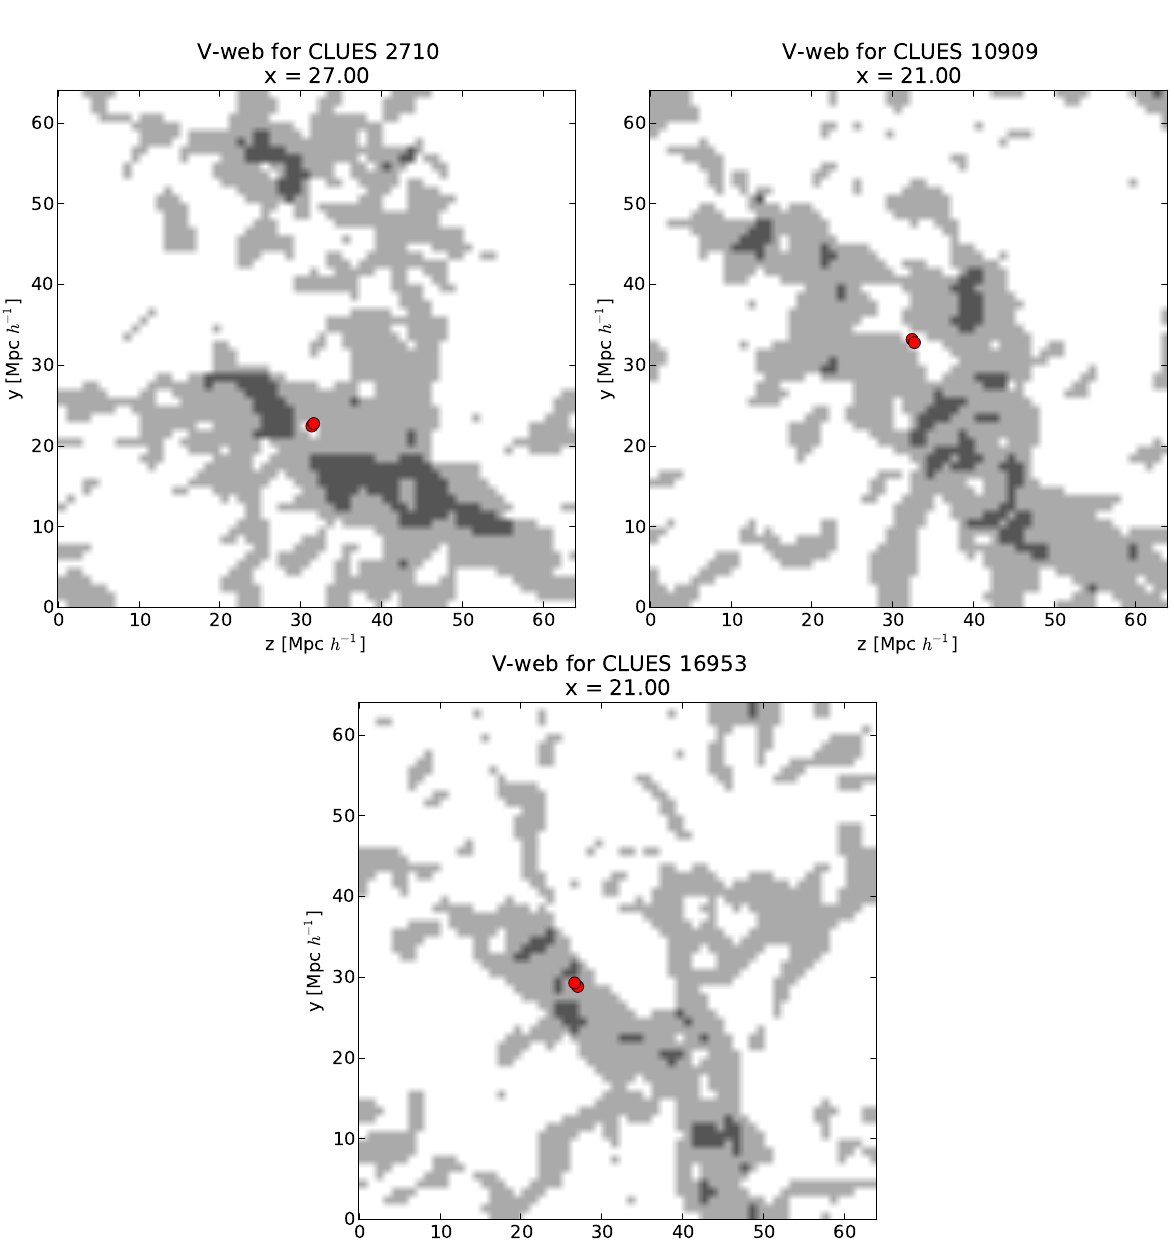
\includegraphics[width=0.75\textwidth]
	{./figures/3_nbody_simulations/LG_Environment.png}

	\caption{\small{Entorno cosmológico a partir del esquema V-web (con 
	$\lambda_{th} = 0.3$) para 	cada uno de los LG de las simulaciones 
	CLUES, indicados por los puntos	rojos.}}
	\label{fig:LG_Sample_Environment}
\end{minipage}
\end{flushright}
\end{figure}
%.........................................................................


Finalmente, a partir de los autovalores extremos hallados se define la 
muestra \textit{CLG} como aquellos pares \textit{IP} cuyos autovalores 
de entorno asociados se encuentran en el intervalo fijado. Para garantizar
autoconsistencia, esta muestra también es definida en las simulaciones 
CLUES.

\end{itemize}
%.........................................................................


%.........................................................................
%Table of samples numbers
\begin{table}[htbp]
\begin{small}
  \centering
  \begin{tabular}{| c | c | c | c | c |} \hline
	\cellc{\textbf{Muestra}}		& 
	\cellc{\textbf{CLUES 1}}		& 
	\cellc{\textbf{CLUES 2}} 		& 
	\cellc{\textbf{CLUES 3}}		& 
	\cellc{\textbf{Bolshoi}}		 \\ \hline
	\textit{GH} 	& 56632 & 57707 & 56799  & 432000 	\\
	\textit{IH}		& 1493 	& 1490 	& 1493	 & 88068 	\\
	\textit{P}		& 386 	& 380 	& 387	 & 23037 	\\
	\textit{IP}		& 20 	& 12 	& 18 	 & 1256 	\\
	\textit{LG}		& 1 	& 1 	& 1 	 & --		\\
	\textit{CLG}	& 1 	& 2 	& 3 	 & 30		\\ \hline
  \end{tabular}
  
  \caption{Tamaños de las muestras definidas para cada una de las 
  simulaciones. }  
  \label{tab:Samples}
\end{small}
\end{table}
%.........................................................................


Para finalizar, en la tabla \ref{tab:Samples} se tabula el tamaño de cada 
una de las muestras definidas para cada simulación. Puede notarse que 
los tamaños escalan aproxi\-madamente en la misma proporción que el 
volumen entre las simulaciones ($1/60$ -- CLUES /Bolshoi). En especial 
la muestra \textit{CLG} para Bolshoi tiene un tamaño proporcional
a la muestra \textit{LG} de las CLUES, indicando que el esquema de 
construcción propuesto reproduce sistemas tipo LG en simulaciones no 
restringidas.


	%---------------------------------------------------------------------
	%Sample Detection Method
	\subsection{Método de Detección de Pares}
	\label{subsec:Pairs_Detection}
	%---------------------------------------------------------------------
	

A continuación se describe el algoritmo desarrollado para la detección de 
cada una de las muestras de pares en cada simulación (\texttt{Pair Finder})
\footnote{Una versión actualizada del código puede encontrarse en 
\url{https://github.com/sbustamante/Thesis/tree/master/codes/Halo_Finder}}.

%.........................................................................
%Algorithm of pair finder
\begin{itemize}
\item Se particiona el espacio de la simulación en $N\times N \times N$
celdas, luego para cada celda se realiza un indexado de los halos que están 
dentro de ella, almacenando los identificadores de cada uno de ellos.

\item Posteriormente, para cada una de las celdas se identifican los 
primeros vecinos, teniendo en cuenta condiciones de frontera periódicas,
tal como la celda $i$ en la figura \ref{fig:Pair_Finder}.

\item Para un halo de una celda dada se calcula la distancia a todos los
halos de la misma celda y de las celdas vecinas, luego se almacena la 
distancia al halo más cercano, la distancia al halo más cercano con una 
masa mayor y la distancia al halo más cercano con una masa mayor a 
$5.0 \times 10^{13}\Msun$.

\item Repitiendo el anterior paso para todos los halos, si dos halos son
mutuamente los dos más cercanos, estos se catalogan como un par, 
construyendo así la muestra \textit{P} definida en la subsección anterior 
\ref{subsec:SampleOfPairsToUse}.

\item Finalmente, para cada uno de los sistemas de pares se evalúan las 
condiciones definitorias de los \textit{IP}, determinando así esta 
muestra.
\end{itemize}
%.........................................................................


%.........................................................................
%Pair Finder Diagram
\begin{figure}[htbp]
	\centering
	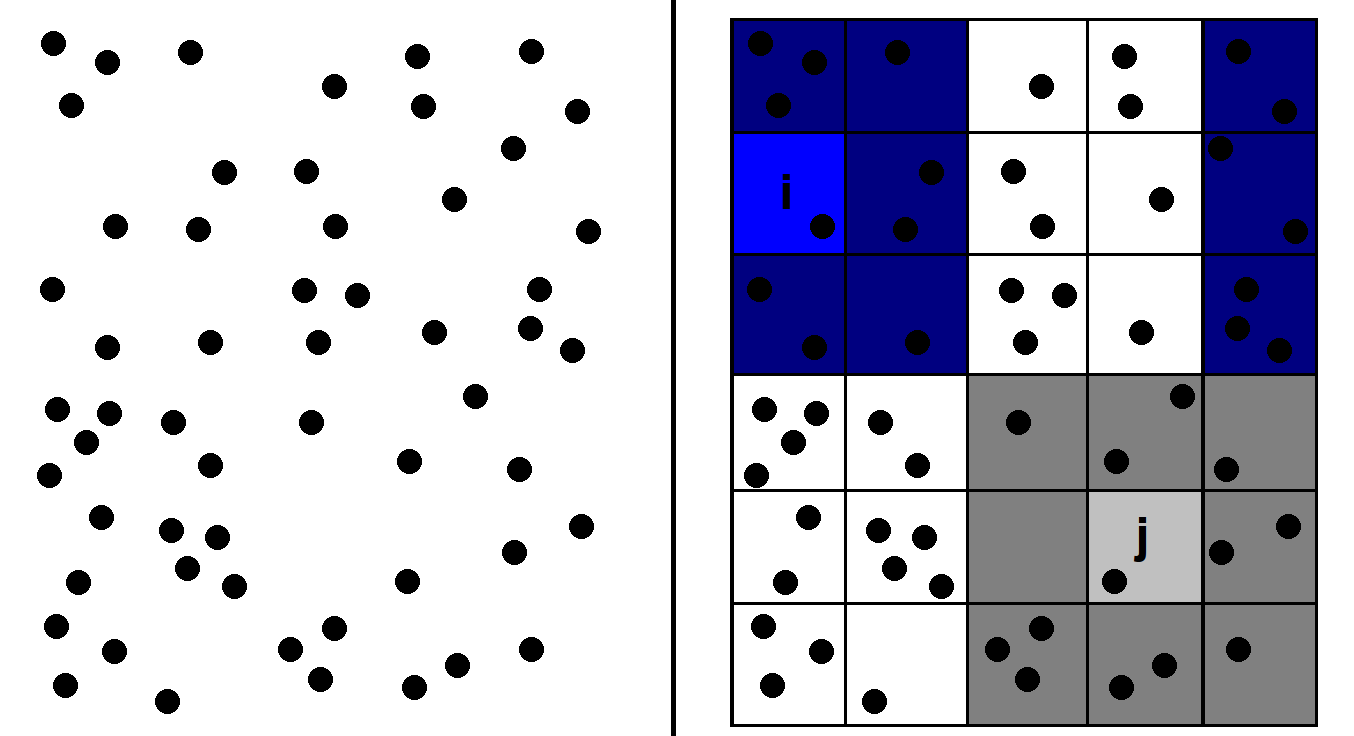
\includegraphics[width=0.6\textwidth]
	{./figures/3_nbody_simulations/PairFinder.png}

	\caption{\small{Ilustración 2D del método para la detección de las 
	muestras de pares. Distribución de halos de materia oscura (izquierda), 
	definición de zonas (derecha).}}
	\label{fig:Pair_Finder}
\end{figure}
%.........................................................................


La eficiencia de este método radica en que evita evaluar distancias entre 
todos los halos de la simulación, siendo necesario solo para los 
vecinos cercanos. La estructura de celdas lo hace similar a un 
código de árbol (ver subsección \ref{subsec:P3Method}), a excepción de la 
estructura jerárquica de este último. En principio, el código debe ser más
eficiente a medida que se aumenta la resolución $N$ de la malla, pero 
existen dos limitaciones que a esto. La primera tiene que ver con el 
número de halos por celda, este no puede ser demasiado grande, pero tampoco 
puede ser tal que solo hallan unos pocos halos por celda \footnote{Este
umbral no es bien definido y depende de cada simulación, por ejemplo para
las simulaciones usadas (Bolshoi y CLUES), un valor de $N=8$ es generalmente 
adecuado.}. La segunda limitación tiene que ver con las condiciones de 
distancia usadas en la definición de la muestra \textit{IP}, el tamaño 
físico de cada celda no puede ser menor a ninguna de estas distancias.


%*************************************************************************